\chapter{La Reacció Química}

Aquest capítol està basat en \citep{caamano_ros_quimica_1991,yen_chemistry_2008,dickerson_principios_1993}.

\section{Termodinàmica Química}

Les reaccions químiques poden ser, a nivell del calor que intercanvien amb l'entorn:
\begin{description}
\item[exotèrmiques] si desprenen calor i, per tant, l'energia dels productes és més baixa que la dels reactius; o bé
\item[endotèrmiques] si l'absorbeixen i els productes acaben tenint més energia que els reactius.
\end{description}

En moltes ocasions mirem d'obtenir treball a partir de la calor produïda en una reacció, com succeix, per exemple, en un procés de combustió o en les reaccions electroquímiques que fan funcionar motors de combustió o elèctrics.

La termodinàmica estudia les relacions entre energia, calor i treball.
En aquest capítol treballarem al voltant de la termoquímica, la termodinàmica associada a les reaccions químiques. 


\subsection{Sistemes, estats i funcions d'estat}

Anomenem "sistema" a aquella part de l'"univers" que volem tractar en algun càlcul o experiment. 
Per exemple, un sistema pot ser un cilindre en un motor de combustió o bé una bateria elèctrica.
\begin{center}
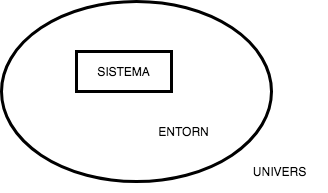
\includegraphics[scale=1.0]{SistEntornUnivers.png}
\end{center}
La resta de l'univers, que no tractem directament, l'anomenarem "entorn".

L'\textit{estat del sistema} es caracteritza  per unes determinades \textit{variables d'estat} ($P$, $V$, $T$, $E$, $H$,...), que són magnituds físiques macroscòpiques mesurables. La termodinàmica estudia els \textit{estats d'equilibri} dels sistemes, en els quals les variables d'estat són idèntiques en totes les seves parts i invariables en el temps.
Tenen dues característiques principals:
\begin{enumerate}
\item En els \textit{canvis d'estat} d'un sistema, les variables d'estat només depenen de l'estat inicial i final, i no del camí utilitzat. Així, per exemple, el treball $W$ no és funció d'estat, mentre que l'energia $E$ sí que ho és.
\item El fet de fixar els valors d'algunes d'elles, una equació d'estat determina automàticament el valor de les altres. Així, com vam veure a la Secció \ref{sec:gasos}
\end{enumerate}

Els canvis d'estat poden ser 
\begin{description}
\item[reversibles] quan les funcions d'estat varian de manera infinitessimal, mantenint el sistema constantment en l'equilibri (l'expansió d'un gas contra una pressió que difereix només $dP$ de la pressió interna, per exemple);
\item[irreversibles] en qualsevol altre situació (un procés de combustió, l'expansió d'un gas contra el buit, etc).
\end{description}


\subsection{Treball}

El treball realitzat per una força en desplaçar un cos entre dues posicions es calcula segons:
\[
w=\int_{x_1}^{x_2} \vec{F} \cdot \vec{dx}
\]
Tenint en compte que $P=\frac{F}{A}$, és fàcil veure que, en el cas d'un pistó que exerceixi una pressió externa sobre un gas 
\begin{center}
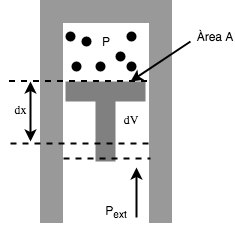
\includegraphics[scale=0.8]{pisto_dw.png}
\end{center}
tenim
\[
dw=-F_{ext}dx = -P_{ext} A dx = -P_{ext} dV
\]
i, per tant,
\[
w=-\int_{V_1}^{V_2} P_{ext} dV
\]
\begin{exr}
Calcula el treball realitzat per comprimir un gas a pressió constant entre un volum inicial $V_1$ i un volum final $V_2$.
\begin{center}
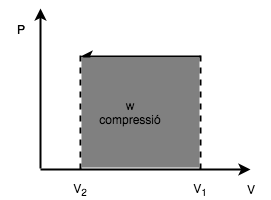
\includegraphics[scale=0.8]{wV.png}
\end{center}
\end{exr}
\begin{exr}
Calcula el treball per dur un gas en un cilindre amb un èmbol des d'un estat de pressió 2 atm i volum 10 l fins a un estat de pressió 5 atm i volum 15 l per dos camins diferents:
\begin{enumerate}
\item Primer escalfant el gas a volum constant i després alliberant l'èmbol a pressió externa constant fins al volum desitjat.
\item Segon deixant l'èmbol lliure (pressió externa constant) mentre escalfem el gas, seguit de continuar escalfant fins que arribem a la pressió objectiu.  
\end{enumerate}
\end{exr}
\begin{exr}
\begin{itemize}
\item Calcular el treball d'expansió reversible i isotèrmic, a 25$\degree$C, de 3 mols d'un gas ideal entre 2 i 3 l de volum.
\item I si es tracta d'un procés irreversible?
\item Repeteix els dos apartats anteriors per a un procés de compressió entre 3 i 2 l del mateix gas.
\end{itemize}
\end{exr}

Dels exercicis anteriors es despèns que el treball no és una funció d'estat.

\subsection{Calor}

La calor $q$ és una magnitud macroscòpica que representa l'efecte d'infinitud de treballs microscòpics deguts als moviments de les partícules d'un sistema.
Com el treball, no és una funció d'estat, ja que depèn del camí que utilitzem per transferir-lo.
La Calor es medeix en calories o Joules.

La quantitat de calor necessària per incrementar la temperatura un determinat valor és\marginnote{Definim com caloria la quantitat de calor necessària per escalfar 1 gr d'aigua 1$\degree$C. Per tant, la capacitat calorífica de l'aigua és $C_p=1 cal g^{-1} \degree C^{-1}$. En realitat, això només és cert per a una temperatura donada, ja que la capacitat calorífica depèn lleugerament de la temperatura de partida. En el cas de l'aigua, la caloria es defineix per al pas de 14.5$\degree$C a 15.5$\degree$C. La quantitat de treball necessària per produir aquesta calor es va determinar per Mayer y Joule el s. XIX com $1cal=4.1860J$. En química usem més sovint les Capacitats calorífiques molars, $C_m$,  que indiquen la quantitat de calor necessària per escalfar un mol d'una substància 1$\degree$C.}
\[
q=nC_m\Delta T
\]
Si aquesta expressió la usem per explicar un procés infinitessimal obtenim
\[
C_m=\frac{1}{n}\frac{dq}{dT}
\]
I com que la capacitat calorífica es pot obtenir a $V=cnt$ o a $P=cnt$, podem calcular
\[
q_v=\int_{T_1}^{T_2} n C_{v,m} dT
\]
i
\[
q_p=\int_{T_1}^{T_2} n C_{p,m} dT
\]

\subsection{Primera llei de la termodinàmica: calor, treball i energia}

Podem incrementar l'energia d'un sistema afegint-hi calor o bé treball. A partir del fet que l'energia es conserva (o, el que és el mateix, que l'energia de l'univers és constant), podem veure que, si obviem l'energia potencial o cinètica global del sistema (l'anomenada energia externa) 
\[
q+w=\Delta U
\]
on $U$ és l'energia interna del sistema, que és funció d'estat!
Aquesta energia interna es pot desglossar en l'energia $U_0$ de les molècules a $T=0K$, sense cap moviment, l'energia tèrmica $U_{term}$ deguda al moviment de les molècules per la temperatura i l'energia potencial intermolecular $U_p$:
\[
U=U_0+U_{term}+U_p
\]
on $U_0$ es pot calcular a partir de càlculs moleculars i es desglossa en 
\begin{enumerate}
\item energia de traslació,
\item energia de rotació,
\item energia de rotació, i 
\item energia electrònica.
\end{enumerate}
\begin{exr}
A partir de l'expressió de l'energia cinètica mitja de les molècules d'un gas ideal, calcula l'energia de traslació que tindrà aquest gas a 298 K.
\end{exr}
\begin{exr}
Quina calor se li ha de donar a un gas ideal perquè s'expandeixi de manera reversible i isotèrmica de $V_1$ a $V_2$ ($V_2>V_1$)?
%l'energia interna només depèn de la temperatura. Per tant, aquí $\Delta U=0$. Per tant, $q=-w$ i podem integrar entre els dos volums per obtenir el resultat.
\end{exr}
En absència de treball útil (elèctric, per exemple, a partir d'una reacció química), $q_V=\Delta U$.
Si el procés té lloc a pressió constant:
\[
q_P  -P\Delta V = (\Delta U)_P
\]
Podem definir una nova funció entalpia com $H=U+pV$.
Aleshores:
\[
\Delta H = \Delta U + \Delta(PV)
\]
a pressió constant és fàcil veure que
\[
(\Delta H)_P = (\Delta U)_P + P\Delta V
\]
i que 
\[
q_P=(\Delta H)_P 
\]
Per tant:
\begin{itemize}
\item la calor transferida a volum constant és igual a l'increment d'energia interna del sistema, i
\item la calor transferida a pressió constant és igual a l'increment d'entalpia  del sistema
\end{itemize}

\paragraph{Calor transferida en una reacció química}
Es pot usar una bomba calorimètrica (Figura \ref{fig:Bomb_calorimeter_scheme}) per mesurar la calor transferida a volum constant en una reacció química.
\begin{figure}[h]
\centering
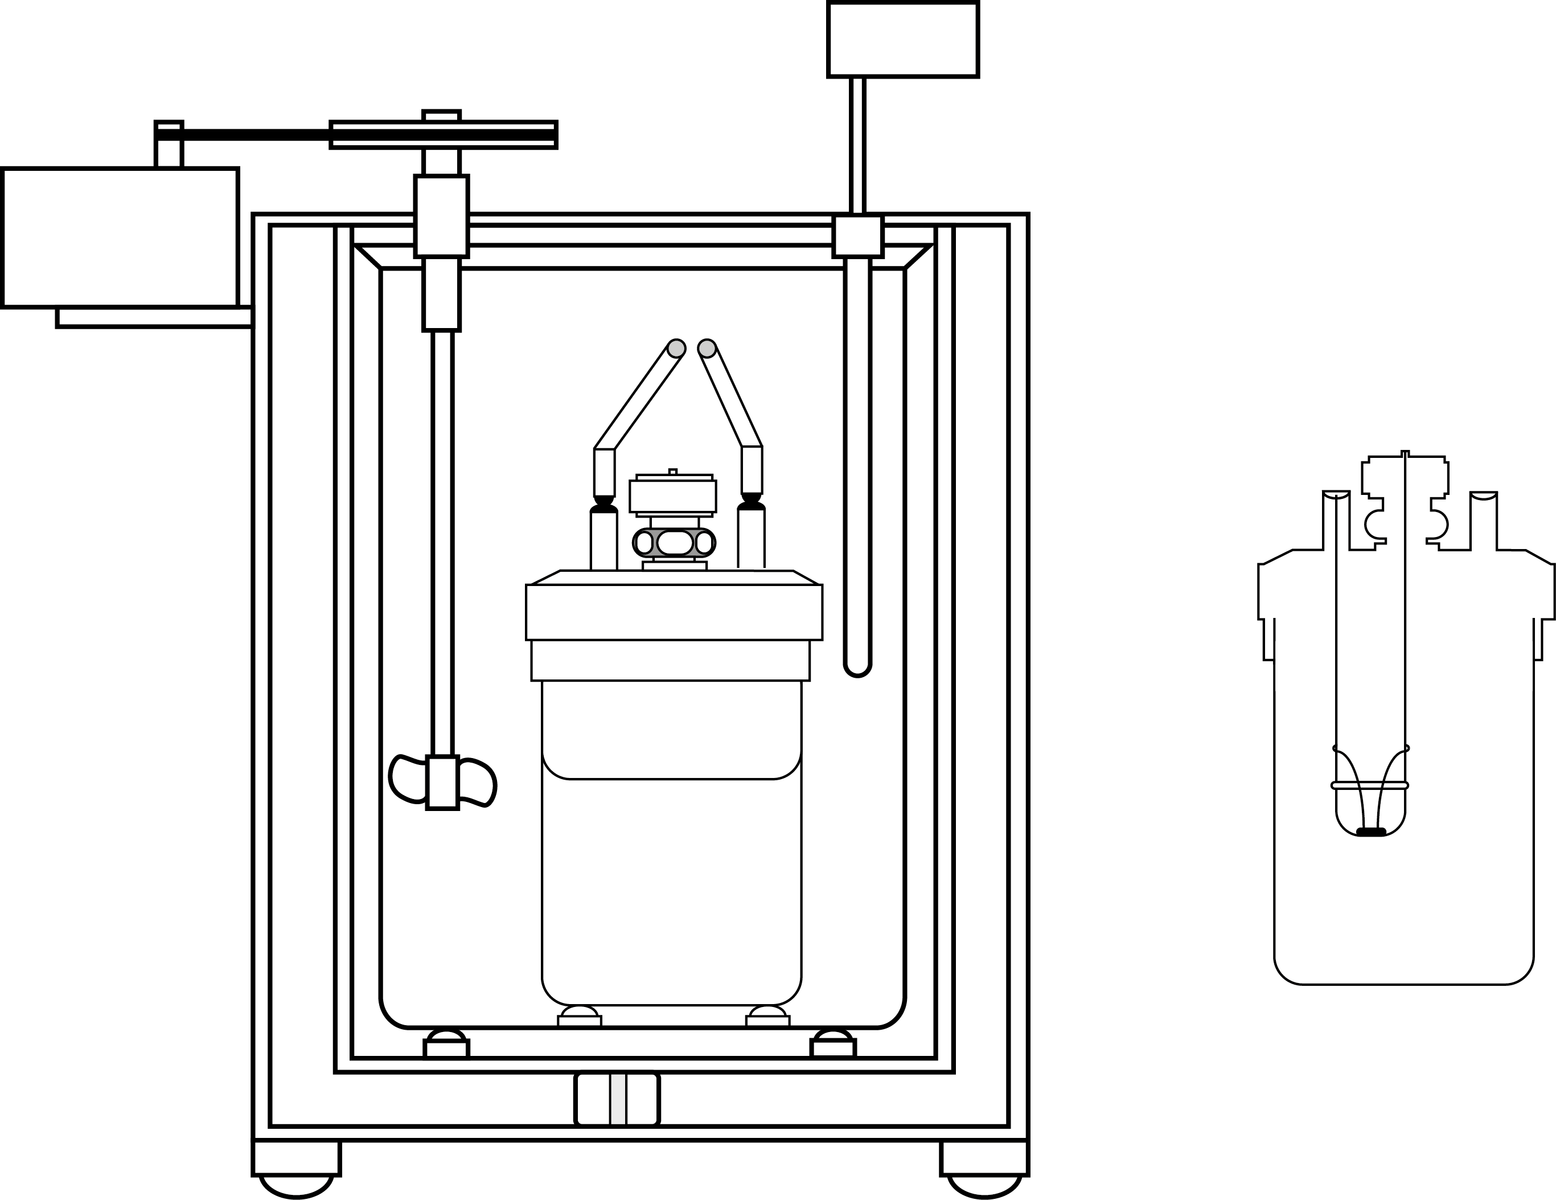
\includegraphics[scale=0.5]{Bomb_calorimeter_scheme.png}
\caption{Bomba calorimètrica.}
\label{fig:Bomb_calorimeter_scheme}
\end{figure}

\begin{exr}
La calor despresa a pressió constant en la combustió del grafit a 298 K i 1 atm és de -110.52 KJ mol$^{-1}$. Si el volum molar del grafit és de 5.3 cm$^3$ mol$^{-1}$, quina és la variació d'energia interna de la mateixa reacció?
% veure exemple 4 de la pàgina 16 del \citep{Caamano1977} III
%\includegraphics[scale=0.5]{ex_grafit.png}
\end{exr}

La calor normal de reacció, $\Delta H^{\circ}$ es defineix com l'entalpia de la reacció a 298 K entre els estats normals de reactius i els estats normals de productes.
Els estats normals es defineixen com:
\begin{itemize}
\item Per a un gas, quan t´una pressió parcial d'1 atm.
\item Per a un líquid, quan és pur en la seva forma més estable a 1 atm.
\item Per a un sòlid, la seva forma més estable a 1 atm.
\item Per a un solut, quan forma una disolució ideal en una concentració de 1 mol dm$^{-3}$.
\end{itemize}
D'aquí podem extreure les calors normals de formació $\Delta H_f^{\circ}$de les diferents substàncies com les calors normals de reacció de la seva formació a partir dels seus elements, cadascun en el seu estat normal.
A partir de les calors normals de formació podem avaluar les calors normals de qualsevol reacció.
\begin{exr}
Calcula la calor normal de la reacció 
\ch{Fe2O3_{(s)}  + 3 H2_{(g)} <-> 2 Fe_{(s)} + 3 H2O_{(aq)}}
\end{exr}

\subsection{Segona llei de la termodinàmica: Entropia}

La primera lei de la termodinàmica estableix que l'energia es conserva en tots els processos ordinaris, però no imposa la direcció de les transformacions de l'energia.
No obstant, hi ha certs processos que sabem que succeeixen de forma espontània, com el traspàs de calor d'un cos calent a un cos fred.
També sabem que no és possible fer una transformació total de l'energia tèrmica a la mecànica, i per tant les diferents formes de l'energia tenen qualitats diferents (Figura \ref{fig:Equality}).
\begin{figure}[h]
\centering
\includegraphics[scale=0.10]{Equality.png}
\caption{Qualitat de la conversió d'energia entre diferents fonts.\citep{yen_chemistry_2008}}
\label{fig:Equality}
\end{figure}

Per tal de mesurar aquest grau d'espontaneïtat dels processos es va desenvolupar el concepte d'entropia. Per a un sistema determinat que pot accedir a diversos nivells d'energia possibles, l'entropia es defineix, a nivell microscopi, com el producte de la constant de Boltzmann amb el logaritme de la probabilitat de maneres d'organitzar els estats d'acord amb un valor accessible d'energia.
\[
S=k \ln \Omega
\]
A nivell macroscòpic, la variació de l'entropia es pot avaluar com la relació entre la calor subministrada de forma reversible a un sistema dividit per la temperatura del procés:
\[
\Delta S = \frac{q_{rev}}{T}
\]
Si la calor es subministra irrevesiblement, sempre tindrem 
\[
\Delta S > \frac{q_{irev}}{T}
\]
A la natura, els processos tendeixen a passar en la direcció de maximitzar l'entropia.
Les formes d'energia que tenen menor quantitat d'entropia per unitat d'energia tendeixen a transformar-se en formes d'energia amb major valor d'aquesta quantitat

\begin{table}[h!]
  \begin{center}
    \caption{Degradació de la qualitat de l'energia en l'univers. Aquest no ''sobreviu'' per cap estabilitat inherent sinó per la successió de ''troballes'' aparentment accidentals, d'obstacles, que arresten el procés normal de degradació de l'energia (adaptat de \citep{dyson_energy_1971}).}
    \label{tab:DegradacioEnergia}
       \begin{tabular}{cc}
Forma de l'energia & Entropia per unitat d'energia\\
\hline
Gravitacional & 0 \\
Nuclear & 10$^{-6}$ \\
Calor interna de les estrelles & 10$^{-3}$ \\
Llum solar & 1 \\
Reaccions químiques & 1-10 \\
Calor de la terra & 10-100 \\
Radiació còsmica de microones & 10$^4$ \\
\hline
       \end{tabular}
   \end{center}
\end{table}

\begin{figure}[h]
\centering
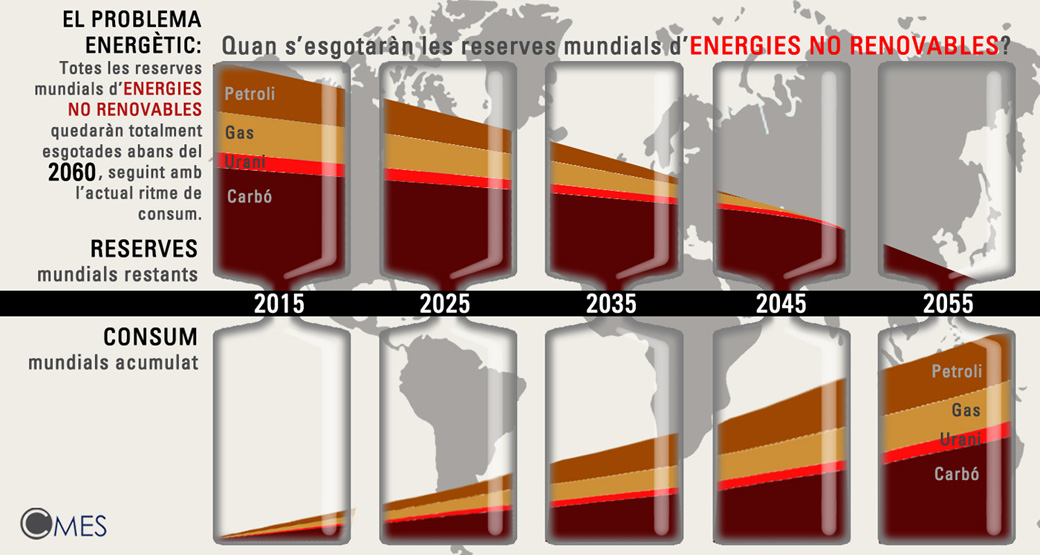
\includegraphics[scale=0.8]{EsgotamentEnergia.png}
\caption{Les crisis energètiques no són conseqüència de la manca d'energia, ja que no pot ser creada ni destruïda. Provenen de la degradació de l'energia entre un estat de gran qualitat a un estat de baixa qualitat. El consum d'energia química provinent de fons fòssils es justifica per la facilitat de la seva explotació, però no per la seva qualitat en termes d'entropia (font Col·lectiu CMES).}
\label{fig:EsgotamentEnergia}
\end{figure}

\subsection{La tercera llei de la termodinàmica}

L'entropia d'un cristall perfecte a zero absolut és zero.

Aquesta llei ens ajuda a posar un valor de referència per a totes les substàncies químiques, permetent-nos construir taules de comparació entre elles. 

\begin{figure}[h]
\centering
\includegraphics[scale=0.1]{EntropyPT2.png}
\caption{Tendències del valor de l'entropia normal (en cal grad$^{-1}$ mol$^{-1}$) per a diferents elements de la taula periòdica.\citep{dickerson_principios_1993}}
\label{fig:EntropyPT2}
\end{figure}

\begin{figure}[h]
\centering
\includegraphics[scale=1]{EntropyTendency.png}
\caption{Tendències del valor de l'entropia normal (en cal $\degree ^{-1} mol^{-1}$) per a diferents propietats físiques de les substàncies.\citep{dickerson_principios_1993}}
\label{fig:EntropyTendency}
\end{figure}

\begin{exr}
\begin{center}
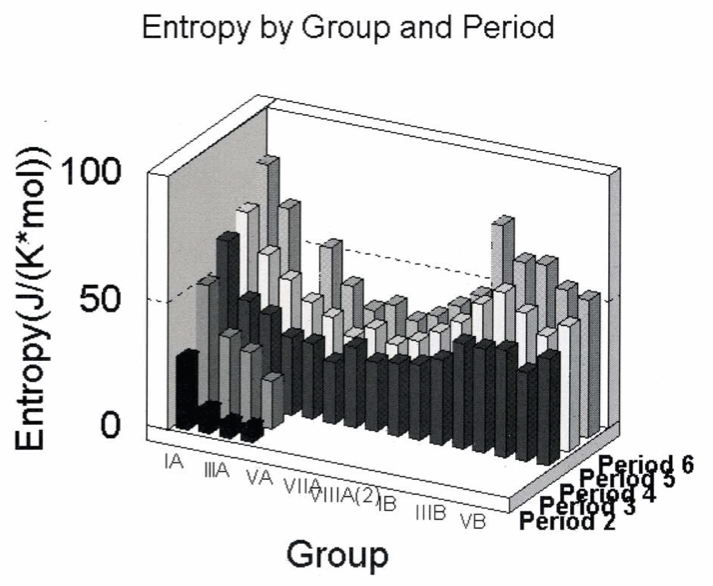
\includegraphics[scale=0.8]{EntropyPT.png}
\end{center}

La Figura mostra l'entropia normal $S^{\circ}_{298}$ per a elements de la taula periòdica, exclosos elements poliatòmics i que no formen sòlids.\citep{thoms_periodic_1995} Pots explicar:
\begin{enumerate}
\item perquè l'entropia augmenta en augmentar el període ($n$ més gran);
\item perquè l'entropia decreix al centre de cada període;i
\item quin és l'efecte d'un augmemnt de l'empaquetament o del grau de coordinació dels elements en l'entropia?
\end{enumerate}
\end{exr}

\section{Espontaneïtat i equilibri químic}

\subsection{Energia lliure}

Per entendre com l'increment d'entropia de l'univers com a criteri d'espontaneïtat dels processos ens pot servir per estudiar l'espontaneïtat dels processos químics cal tornar a discriminar entre el nostre sistema i l'entorn, com hem fet des de l'inici del capítol:
\begin{eqnarray*}
\Delta S_{univers} &= &\Delta S_{sistema} + \Delta S_{entorn}\\
&=&\Delta S_{sistema} + \frac{q_{entorn}}{T}\\
&\geq & 0
\end{eqnarray*}

Pel fet que
\[
\Delta H= q_{sistema} = -q_{entorn}
\]
aleshores
\[
\Delta S_{univers} = \Delta S_{sistema} - \frac{\Delta H}{T} \geq 0
\]
Multiplicat a ambdós costats per $-T$ obtenim l'expressió de l'energia lliure (o energia de Gibbs, nova funció d'estat $G=H-TS$):
\begin{equation}
-T \Delta S_{univers} = \Delta H_{sistema} -T\Delta S_{sistema}= \Delta G_{sistema} \geq 0
\label{Eq:Gibbs}
\end{equation}
El signe de $\Delta G$ determina, doncs, l'espontaneïtat d'una reacció.

Podem relacionar $\Delta G$ amb el treball útil fent unes simples transformacions. Per exemple, si s'aplica treball extern sobre el sistema de forma reversible (quan $q-T\Delta S=0$) tot el treball extern diferent de l'usat per variar el volum del sistema es transforma en variació d'energia lliure:
\[w=P\Delta V + w_{ext}\]
\[\Delta E = q-P\Delta V -\w_{ext}\]
\[\Delta H= q-w_{ext}\]
\[\delta G = q - T\Delta S -w_{ext} = -w_{ext}\]
Així, en una cel·la electroquímica, com veurem, el treball realitzat per la cèl·lula és una mesura directa del descens 
d'energia lliure dins seu. Alternativament, si apliquem potencial elèctric entre els terminals d'una cel·la d'electròlisi el treball elèctric realitzat sobre la cel·la és identic a l'augment d'energia lliure dels productes químics que conté. Per exemple, si dissociem electrolíticament l'aigua augementem l'energia lliure dels seus components hidrogen i oxigen, energia que podem recuperar després:
\[\ch{H2O_{(l)]} -> H2_{(g)} + 1/2 O2_{(g)}} \quad \Delta G^{\circ}= 56.69 kcal mol^{-1}\]
La clau rau en que aquesta trasformació posterior resulti en el mínim de calor i el màxim de treball.

\subsection{Càlcul de les energies lliures normals}

A partir de les dades tabulades en diverses fonts de l'entalpia normal de formació i l'entropia normal de cada ubstància, respectivament, podem calcular els valors de qualsevol procés químic.
\begin{exr}
Calcula l'energia lliure, l'entalpia i l'entropia normals per a la reacció \ch{3 H2_{(g)} + N2_{(g)} -> 2 NH3_{(g)}}. Què afavoreix i què desafavoreix la reacció? Succeiria igual a qualsevol temperatura?
%\includegraphics[scale=0.8]{exdG.png}
\end{exr}

\begin{exr}
Calcular els canvis d'energia lliure, entalpia i entropia per a la vaporització de l'aigua líquida. Quina influència hi té la pressió de vapor de l'aigua?
\end{exr}

\subsection{La natura de l'equilibri químic}

Les reaccions químiques són reversibles i, per aquest fet, els sistemes químics tancats produeixen un equilibri entre reactius i productes.
En aquest apartat relacionarem l'estructura atòmica de la matèria amb la tendència i l'espontaneïtat descrites en els apartats anteriors.

En la Figura \ref{fig:evap_vs_condens} vam introduir el concepte de reversibilitat d'un procés d'evaporació. Aquest fenòmen, eminentment físic, conduïa a un estat d'equilibri entre dues fases, que implicava la conservació d'aquestes però no pas de les molècules individuals que les formaven, les quals anaven fluctuant entre les dues fases.
El mateix succeeix en els processos químics. 
Posem per cas la reacció de descomposició tèrmica del carbonat de calci:
\[
\ch{CaCO3_{(s)} -> CaO_{(s)} + CO2_{(g)}}
\]
Aquesta reacció pot dur-se a terme fins a la descomposició total del \ch{CaCO3} si usem algun sistema per arrastrar el \ch{CO2} que es va formant. En canvi, sabem que si la pressió de \ch{CO2} en un recipient tancat que conté \ch{CaO} és prou alta, acabem formant de nou \ch{CaCO3}. Per tant, la reacció s'ha d'escriure, millor, fent:
\[
\ch{CaCO3_{(s)} <=> CaO_{(s)} + CO2_{(g)}}
\]
que indica que els reactius i productes assoleixen un equilibri en determinades condicions. Com vam veure a la Secció \ref{sec:PropietatsCritiques}, 
\begin{enumerate}
\item L'equilibri en els sistemes moleculars és dinàmic, conseqüència de velocitats de reacció oposades.
\item El sistema passa espontàniament a l'estat d'equilibri.
\item Un cop assolit l'equilibri, les seves propietats són sempre les mateixes.
\item L'equilibri és fruit de dues tendències oposades: la necessitat d'assolir el mínim d'energia i la tendència al màxim caos.
\end{enumerate}
Amb el què hem anat veient en les darreres seccions, algunes d'aquestes propietats adquireixen nou sentit.
\begin{enumerate}
\item Si volem comprovar que l'equuilibri és dinàmic només cal usar \ch{CO2} etiquetat radioactivament (és a dir, que contingui un isòtop radioactiu que poguem detectar, com el \ch{^{14}C}). Al cap d'una estona comprovarem que part d'aquest \ch{^{14}C} s'ha incorporat al sòlid en forma de \ch{Ca^{14}CO3}.
\item Quan parlem de tendència espontània a l'equilibri, cal no confondre amb la velocitat amb que això pot succeir. Per a la reacció que estem estudiant,
\[
\Delta G^{\circ} = 177,100 - 158 T \quad J \cdot mol^{-1}
\]
Per tant, a $T$ baixes la reacció no és espontània i sí en canvi a $T$ altes, com es mostra al gràfic:
\begin{center}
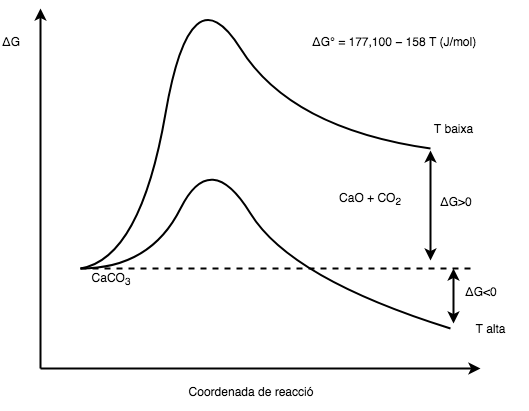
\includegraphics[scale=0.6]{CaCO3_dG.png}
\end{center}
A $T$ altes, segons es pot veure en el gràfic, la barrera d'energia lliure a superar serà més baixa que a $T$ baixes per a a questa reacció, la qual cosa implica que, a més, la reacció serà més ràpida. Però aquest és un concepte cinètic que treballarem més tard.
\item En el nostre exemple, les característiques de les molècules a reactius i productes es mantenen, complint el tercer dels enunciats de més amunt: per a cada $T$ hi ha un valor de la pressió de vapor del ch{CO2} en equilibri. Cal tenir present la molaritat de la reacció química, però (és a dir, el numero de mols que posem . Ho veurem més endavant.
\item Finalment, les dues tendències oposades (la formació de carbonat càlcic a partir de l'addició de diòxid de carboni a l'òxid de calci enfront de la descomposició tèrmica de la primera substància) s'han vist clarament en l'exemple exposat. El gràfic de l'energia lliure mostra també com, en aquest cas en que es desprèn un gas a partir d'un sòlid, el terme entròpic és clarament favorable, mentre que la calor (entalpia) necessària per fer la descomposició és elevada i contrària al procés.
\end{enumerate}

\begin{exr}
Pots racionalitzar qualitativament els quatre factors implicats en la descripció de l'equilibri químic en les reaccions:
\[ \ch{H2_{(g)} <=> 2 H_{(g)}}\]
\[ \ch{H2_{(g)} + I2_{(g)} <=> 2 HI_{(g)}}\]?
Per a les dues reaccions, calcula el valor de $\Delta G^{\circ}$ a partir de dades obtingudes a la literatura (usa els enllaços de la Secció \ref{EnllacosInteres}). 
\end{exr}

\begin{exr}
Com afectaria l'ús d'un catalitzador la corba d'energia lliure que hem dibuixat en el cas de la reacció de descomposició tèrmica del \ch{CaCO3}?
\end{exr}

\subsection{Constant equilibri}

Un cop assolit un equilibri com el de la reacció 
\[ \ch{H2_{(g)} + I2_{(g)} <=> 2 HI_{(g)}}\]
hi ha infinites possibilitats de combinacions de pressions de vapor dels tres gasos, però sempre es complirà, a una $T$ donada, la relació
\[
K=\frac{P^2_{\ch{HI}}}{P_{\ch{H2}}P_{\ch{I2}}}
\]
En general, i per a una reacció en equilibri del tipus
\[
\ch{a A + b B <=> c C + d D}
\]
es complirà, a una $T$ donada
\[
K=\frac{[C]^c[D]^d}{[A]^a[B]^b}
\]
Aquesta constant $K$ només depèn de la $T$ i de les substàncies que intervenen en la reacció. Si algun component és gasos es pot usar la seva pressió de vapor en l'expressió enlloc de la seva concentració.
\begin{exr}
Perquè podem usar la pressió de vapor enlloc de la concentració per a una substància gasosa en l'expressió de la constant d'equilibri?
Succeiria el mateix si el sistema no fos ideal? Serveix l'expressió per a qualsevol concentració de les substàncies reaccionants?
\end{exr}

\begin{exr}
Pots raonar perquè la constant d'equlibri de la descomposició tèrmica del \ch{CaCO3} és igual a $P_{\ch{CO2}}$?
\end{exr}

\begin{exr}
Com afecta la constant d'equilibri el fet d'igualar la reacció química amb coefficients que són els doble o el triple dels escrits inicialment?
\end{exr}

\begin{exr}
Quina és la relació entre la constant d'equilibri d'una reacció i la de la seva inversa?
\end{exr}

\begin{exr}
Escriu la constant d'equilibri de la reacció 
\[\ch{2 NO_{(g)} + O2_{(g)} <=> N2O4_{(g)}}\]
a partir de les de les reaccions 
\[\ch{2 NO_{(g)} + O2_{(g)} <=> 2 NO2_{(g)}}\]
i 
\[\ch{2 NO2_{(g)} + O2_{(g)} <=> N2O4_{(g)}}\]
\end{exr}



A partir de la definició de la constant, és fàcil deduir què és una constant de solubilitat d'una determinada substància, com mostra el següent exercici:

\begin{exr}
Quina és la constant de solubilitat del cromat d'argent (\ch{Ag2CrO4}) si la concentració d'una dissolució saturada d'aquesta sal té una concentració de 6.7$\times$10$^{-5}$M d'ions cromat?
\end{exr}

En general, quan estem dissolent una sal poc soluble, sempre tindrem el sòlid acompanyant els ions dissolts. Així, la concentració del sòlid es podrà considerar incorporada a la constant d'equilibri i parlarem de constants o productes de solubilitat.
Els productes de solubilitat es poden emprar per fer precipitació selectiva d'ions en una dissolució complexa. 

\begin{exr}
S'afegeix ió \ch{Ag+} a una dissolució que conté \ch{Cl-} i \ch{I-}, ambdós a una concentració de 0.01 M. Què precipita abans, \ch{AgCl} i \ch{AgI}. Quina és la concentració d'ions \ch{Ag+} quan la primera sal comença a precipitar? I quina és la concentració de l'anió del primer precipitat quan la segona sal comença a precipitar?
\end{exr}

Finalment, la relació entre la constant d'equilibri i l'energia lliure de la reacció ve donada per
\[\Delta G = -RT ln K_{eq}\]

\subsection{Efectes externs sobre equilibri}

\begin{tcolorbox}[colback=green!5,colframe=green!40!black,title=Constant d'Equilibri]
Aprèn la diferència entre quocient i constant d'equilibri amb la simulació que trobaràs a \linkurl{https://teachchemistry.org/periodical/issues/november-2017/predicting-shifts-in-equilibrium}
\end{tcolorbox}

El principi de Le Chatelier estableix que si un sistema en equilibri és pertorbat o a qualsevol tensió en qualsevol dels factors que determinen aquest equilibri, el sistema reaccionarà de tal manera que disminuirà l'efecte de la pertorbació. 
 Els efectes externs sobre un equilibri es poden entendre amb faciltat pensant en el retorn a la situació d'equilibri des de la què ens hem desplaat. Per exemple:

\begin{itemize}
\item Si augmentem o disminuïm la concentració d'una substància, l'equilibri es desplaçarà cap a formar una nova relació entre components que compleixi el valor de la $K$. La Taula \ref{tab:Eqs} permet visualitzar alguns d'aquests efectes.
\item Si augmentem el volum del sistema (en una reacció en fase gas) no necessàriament canviarem les condicions d'equilibri (dependrà de la molaritat de la reacció).
\item En una reacció endo/exotermica, un augment de la temperatura desplaça l'equilibri cap a la dreta o cap a l'esquerra, respectivament.
\end{itemize}

\begin{exr}
La constant d'equilibri de la reacció d'isomerització entre l'$n$-butà i l'isobutà és 2.5. Representa gràficament la tendència del sistema en funció de diverses concentracions inicials de cadascuna de les dues substàncies. (Pista: representa la pressió de vapor de l'$n$-butà en abcisses i la de l'isobutà en ordenades com mostra la Taula \ref{tab:Eqs}).
\end{exr}

\begin{exr}
Fes una interpretació similar per al cas de la reacció de dissociació del sulfat de bari en els seus components iònics (veure Taula \ref{tab:Eqs}).
\end{exr}

\begin{exr}
La constant d'equilibri de la dissociacio del \ch{NH4HS} sòlid en amoniac i sulfur d'hidrogen és de 0.11 atm$^2$. Si posem una mica d'aquest sòlid en un recipient tancat que conté amoniac a una pressió de 0.5 atm. Quina és la pressió final del sistema un cop assolit l'equlibri?
% pàgina 188 del mahan
\end{exr}

\begin{table}[h!]
  \begin{center}
    \caption{Representació gràfica de processos en equlibri simples. Casos genèrics com \ch{a A + b B <=> c C + d D} són més complexes de visualitzar, però la tendència que segueixen quan els posem lluny de l'equilibri també es pot entendre fàcilment valorant si $\frac{[C]^c[D]^d}{[A]^a[B]^b}<K_{eq}$ o $\frac{[C]^c[D]^d}{[A]^a[B]^b}>K_{eq}$. }
    \label{tab:Eqs}
    \begin{tabular}{c|c}
      \hline
      Tipus de reacció (Exemple) & representació gràfica de l'equilibri \\
      \hline
$\begin{array}{c}\ch{A_{(s)} <=>  A_{(g)}} \\ \ch{CaCO3_{(s)} <=>  CaO_{(s)} + CO2_{(g)}}\end{array}$ &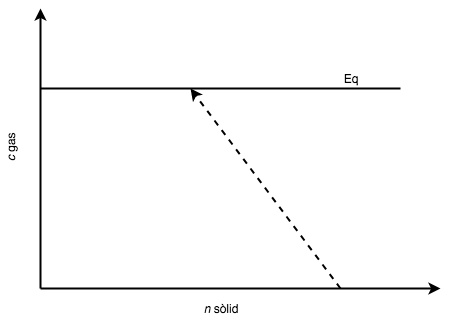
\includegraphics[scale=0.3]{Eq1.png} \\ \hline
$\begin{array}{c}\ch{A <=> B} \\  \ch{n-butà <=> isopropà}\end{array}$ & 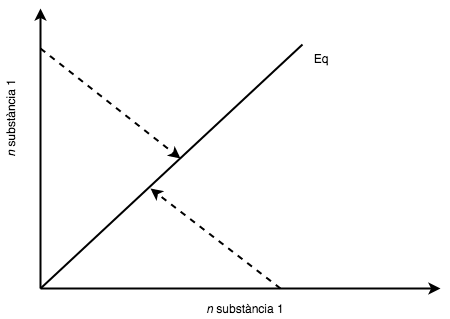
\includegraphics[scale=0.3]{Eq2.png} \\ \hline
$\begin{array}{c}\ch{A_{(s)} <=> B + C} \\ \ch{BaSO4_{(s)} <=>  Ba^{2+}_{(aq)} + SO4^{2-}_{(aq)}}\end{array}$ & 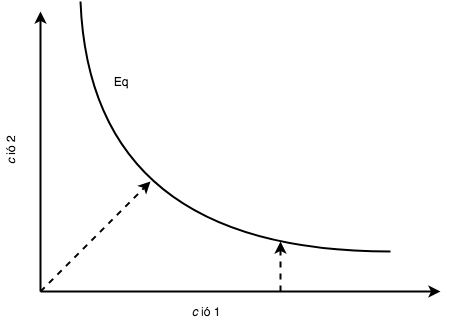
\includegraphics[scale=0.3]{Eq3.png} \\\hline
$\begin{array}{c}\ch{A <=> 2B} \\ \ch{N2O4_{(g)} <=> NO2_{(g)}}\end{array}$ & 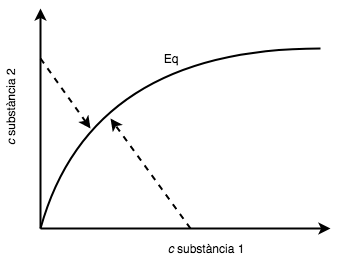
\includegraphics[scale=0.4]{Eq4.png} \\
      \hline
    \end{tabular}
  \end{center}
\end{table}

\begin{exr}
La constant d'equilibri de la reacció
\[
\ch{CO2_{(g)} + H2_{(g)} <=> CO_{(g)} + H2O_{(g)}}
\]
a 690K és 0.10. Quina és la pressió d'equilibri del sistema si barregem 0.5 mol de \ch{CO2} i 0.5 mol de \ch{H2} en un recipient de 5 l a 690K?
Si augmentéssim la T, la pressió augmentaria o disminuiria?
\end{exr}

\subsection{Equilibris no ideals}

En reaccions no ideals (molt concentrades o amb gasos a alta pressió) no podem expressar la constant d'equilibri com a producte de concentracions o pressions parcials, sinó que hem d'usar el concepte activitat. L'activitat de les substàncies dissoltes o dels gasos, en els dos exemples descrits, dependrien de la concentració o la pressió, però serien tan diferents d'aquestes com més allunyades de la idealitat estiguessin. En aquests casos, per a \ch{a A + b B <=> c C + d D}, escrivim:
\[
\frac{a_C^c a_D^d}{a_A^a a_B^b}=K_{eq}
\]

%\subsection{Cinètica química}
%
%\section{Precipitació}
%
\section{Equilibri iònic en solucions aquoses}

\subsection{Reaccions àcid-base}

Un cas de gran interès en química és la comprensió de l'equilibri iònic en dissolucions aquoses. 
Aquest cas particular ens farà comprendre processos àcid base, que formen una gran part de les casuístiques d'interès en la química.

Hi ha tres gran teories que permeten explicar el concepte àcid-base:\marginnote{D'entre els molts recursos disponibles a la xarxa, és particularment simple i ben explicat el que trobareu a \linkurl{https://www.chemguide.co.uk/physical/acidbaseeqia/theories.html}}
\begin{description}
\item[Arrhenius]
Arrhenius (1880-1890) va desenvolupar la teoria segons la qual àcids i bases es dissociaven en els seus ions segons:
\[\ch{\textit{A}H <=> \textit{A^-} + H+}\]
\[\ch{\textit{B}OH <=> \textit{B^+} + OH-}\]
En realitat, l'existència de l'ió \ch{H+} és fictícia, ja que es troba sempre solvatat amb una molècula d'aigua en forma de \ch{H3O+} o estats d'hidratació superior.

\item[Lowry-Br{\o}nsted] Això ens duu de forma natural al concepte d'àcid-base formulat per Lowry-Br{\o}nsted (1923): un àcid és una espècie química amb tendència a donar un protó, i una base a acceptar-lo.
Així, ens queda:
\[\ch{\textit{A}H + \textit{B} <=> \textit{A}^- + \textit{B}H^+}\]

\begin{exr}
Escriu la reacció àcid-base de l'ió carbonat en aigua en equlibri amb l'ió bicarbonat. Qui té el rol d'àcid i de base en la reacció directa i la inversa?
\end{exr}

Per a una reacció àcid-base d'una substpancia acídica en aigua tindríem, per exemple:
\[\ch{HSO4- + H2O <=> H3O+ + SO4^{2-}}\]
A partir d'aquesta expressió, podem escriure la constant d'equilibri, o constant de dissociació de l'àcid $K_a$, de la reacció com\marginnote{\label{foot:KaKb}Pots trobar dades de $K_a$ i $K_b$ a \linkurl{https://chem.libretexts.org/Reference/Reference_Tables/Equilibrium_Constants}}
\[K_a = \frac{[\ch{H3O+}][\ch{SO4^{2-}}]}{[\ch{HSO4-}]}\]

\item[Lewis] Finalment, també podem entendre el concepte d'àcid-base a partir de la definició de Lewis (1923). 
Segons aquesta definició, un àcid és qualsevol substpancia que pot acceptar electrons, i una base és tota substància que en pot donar.
Es tracta d'una definició més genèrica perquè no implica la presència de protons.
\end{description}

Per al que segueix usarem essencialment la definició de Lowry-Br{\o}nsted.

\subsection{L'escala de pH}

La reacció d'equilibri de la hidròlisi de l'aigua es pot escriure com
\[\ch{H20_{(l)} + H20_{(l)} <=> H3O+_{(aq)} + OH-_{(aq)}}\]
i té associada una constant d'equilibri $K_w$:
\[K_w=[\ch{H3O+}][\ch{OH-}]\]
amb un valor de 10$^{-14}$ a 25${\degree}$C si expressem la concentració dels dos ions en $M$.
En aigua pura, doncs, la concentració d'ions \ch{H3O+} i \ch{OH-} és de 10$^{-7}$ M, respectivament. 
Per tal de facilitar els càlculs treballem normalment en escala logarítmica i definim
\[pH = - \log_{10} [\ch{H3O+}]\]
Per tant, un valor de pH=7 implica que tenim una dissolució neutra pel que fa a la seva acidesa. Una concentració superior de protons (pH<7) implica una dissolució àcida i a l'inrevés.
 
\begin{exr}
Quin és el pH d'una dissolució de 0.1 M de clorur d'hidrogen? i d'una d'àcid benzoic a la mateixa concentració?
\end{exr}

És fàcil veure que $K_w=K_a K_b$, que ens diu també que, si l'àcid és fort, la seva base conjugada és feble, i a l'inrevés.

També és fàcilment deduïble l'equació de Henderson-Hasselbalch, que relaciona el pH d'una dissolució àcida amb el pK$_a$ i la concentració d'ions presents:
\[
pH = pK_a + \log_{10} \frac{[A^-]}{[AH]}
\]

\begin{exr}
Els productes de solubilitat de \ch{Fe(OH)3} i \ch{Zn(OH)2} són 4$\cdot$10$^{-38}$ i 4.5$\cdot$10$^{-17}$. A quin pH podem considerar que la precipitació de l'hidròxid de ferro és pràcticament completa mentre que l'ió \ch{Zn^{2+}} queda a una concentració de 0.5 M?
\end{exr}

%\subsection{Solucions reguladores i tampons}
%\subsection{Tractament exacte equuilibris ionització}
%\subsection{	Valoracions}
%

\section{Reaccions REDOX}

Quan observem la taula periòdica, podem apreciar que hi ha elements amb gran capacitat de donar electrons (metalls alcalins i alcalinoterris, per exemple) i anomenem electropositius. 
De la mateixa manera, anomenem electronegatius els elements que tenen gran capacitat d'acceptar electrons.

Definim l'estat d'oxidació d'un àtom com a la suma de càrregues positives i negatives que té. Això dóna idea de la càrrega total que conté.
En l'enllaç iònic que forma el \ch{NaCl}, l'estat d'oxidació del sodi és +1 i del clor -1.
En una molècula, usem els següents criteris per assignar els estats d'oxidació als diferents elements:
\begin{enumerate}
\item L'estat d'oxidació dels elements en qualsevol forma al·lotròpica en què  presentin és zero.
\item L'EO de l'oxigen és zero en tots els seus compostos, excepte en els peròxids (\ch{H2O2}, \ch{Na2O2}).
\item L'EO de l'hidrogen és +1 en tots els compostos, excepte en aquells que forma amb metalls, on és -1.
\item L'EO de la resta d'elements d'una substància s'escullen per tal que la suma de tots ells sigui zero o bé la càrrega que hagi de tenir l'ió que formen.
\end{enumerate}

Així com les reaccions àcid-base impliquen una transferència protònica (com a mínim en la definició de Lowry-Br{\o}nsted que hem estat usant) existeixen reaccions en les quals hi ha una transferència electrònica i que anomenem de Reducció-oxidació (REDOX). En totes aquestes reaccions en les quals participa el zinc hi ha el mateix procés d'oxidació (pèrdua d'electrons) d'aquest element:
\[\ch{Zn + Cu^{2+} <=> Zn^{2+} + Cu}\]
\[\ch{Zn + 1/2 O2 <=> ZnO}\]
\[\ch{Zn + Cl2 <=> ZnCl2}\]
\[\ch{Zn + 2 H^+_{(aq)} <=> Zn^{2+}_{(aq)} + H2}\]
En totes aquestes reaccions, el \ch{Zn} actua com a agent reductor, ja que amb la seva pròpia oxidació redueix l'altra substància. 

\begin{exr}
Són reaccions REDOX
\[\ch{ClO- + NO2- <=> NO3- + Cl-} \]
\[\ch{2 CCl4 + K2CrO4 <=> 2 Cl2CO + CrO2Cl2 + 2 KCl} \]?
\end{exr}


\subsection{Concepte de mitja reacció}

Pel fet que podem identificar, en una reacció REDOX, les substancies que es redueixen i les que s'oxiden, podem també separar la reacció global en els dos processos, ja que ens serà útil per comprendre que, de la mateixa manera que fem amb els elements de la reacció, també ens caldrà igualar el nombre d'electrons que s'intercanvien. Això també implica que una reacció REDOX es pot dividir físicament en dos compartiments i que els elecetrons es poden arribar a compartir amb un conductor, com s'aprecia a la Figura \ref{fig:Galvanic_cell_with_no_cation_flow}.

\begin{figure}[h]
\centering
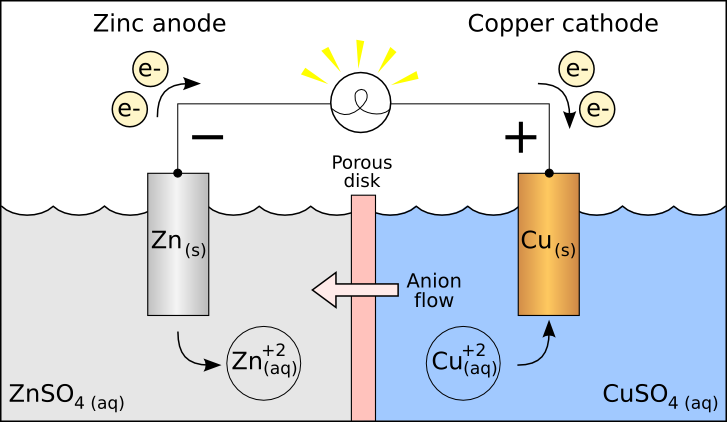
\includegraphics[scale=0.5]{Galvanic_cell_with_no_cation_flow.png}
\caption{Una cel·la galvànica per a la reacció 
\ch{Zn_{(s)} + Cu^{2+}_{(aq)} <=> Cu_{(s)} + Zn^{(2+)}_{(aq)}}. 
La connexió es tanca mitjançant una membrana porosa als ions, però també es podria fer amb un pont salí (tub permeable que conté una dissolució d'alguna sal com \ch{KCl} (\linkurl{https://commons.wikimedia.org/wiki/File:Galvanic_cell_with_no_cation_flow.png})}
\label{fig:Galvanic_cell_with_no_cation_flow}
\end{figure}

En la reacció global representada a la figura hi ha dos processos simultanis, un a cada vas de reacció:
\[\ch{Zn <=> Zn^{(2+)}_{(aq)} + 2 e-}\]
\[\ch{2 e- + Cu^{2+}_{(aq)} <=> Cu_{(s)}}\]
El pont salí fa que es mantingui el balanç de càrregues potivies i negatives a cada vas.


\subsection{Balanç reaccions REDOX}

Separar les dues semireaccions d'una reacció REDOX ajuda a balancejar l'equació global (tenint en compte també els electrons que s'intercanvien) a més de permetre tenir mesures de la tendencia a oxidar/reduir de cada substància.
Per fer el balanç, seguim quatre passos:
\begin{enumerate}
\item Identifiquem les espècies que es redueixen o s'oxiden.
\item Escrivim les dues mitges reaccions.
\item Igualem les dues semireaccions en base als elements i les càrregues.
\item Les sumem per obtenir la reacció global.
\end{enumerate}

\begin{exr}
Iguala la reacció \ch{H2O2 + I- <=> I2 + H2O}. Pista: quan hagis d'afegir hidrogen, fes-ho en forma de protons \ch{H+}.
\end{exr}

\begin{exr}
Iguala la reacció entre en benzaldehid i l'ió \ch{Cr2O7^{2-}} per donar àcid benzoïc i ió \ch{Cr^{+3}}. Pista: on calguin oxigens, afegeix molècules d'aigua; on calguin hidrogens, afegeix protons.
\end{exr}

\begin{exr}
Iguala la reacció \ch{ClO- + CrO2- <=> CrO4- + Cl-} en una dissolució bàsica. Pista: fes com sempre però al final tingues en compte que els reactius han d'incorporar l'ió \ch{OH-}.
\end{exr}

\subsection{Cel·les galvàniques}

Tant en la cel·la galvànica de la Figura \ref{fig:Galvanic_cell_with_no_cation_flow} com en la bateria d'ió Liti de la Figura \ref{fig:LiIon3}, aprofitem el potencial REDOX de les substàncies per tal d'acumular energia química i transformar-la en elèctrica. 
Anomenarem càtode a l'enectrode on té lloc la reducció i ànode on té lloc l'oxidació.

\begin{figure}[h]
\centering
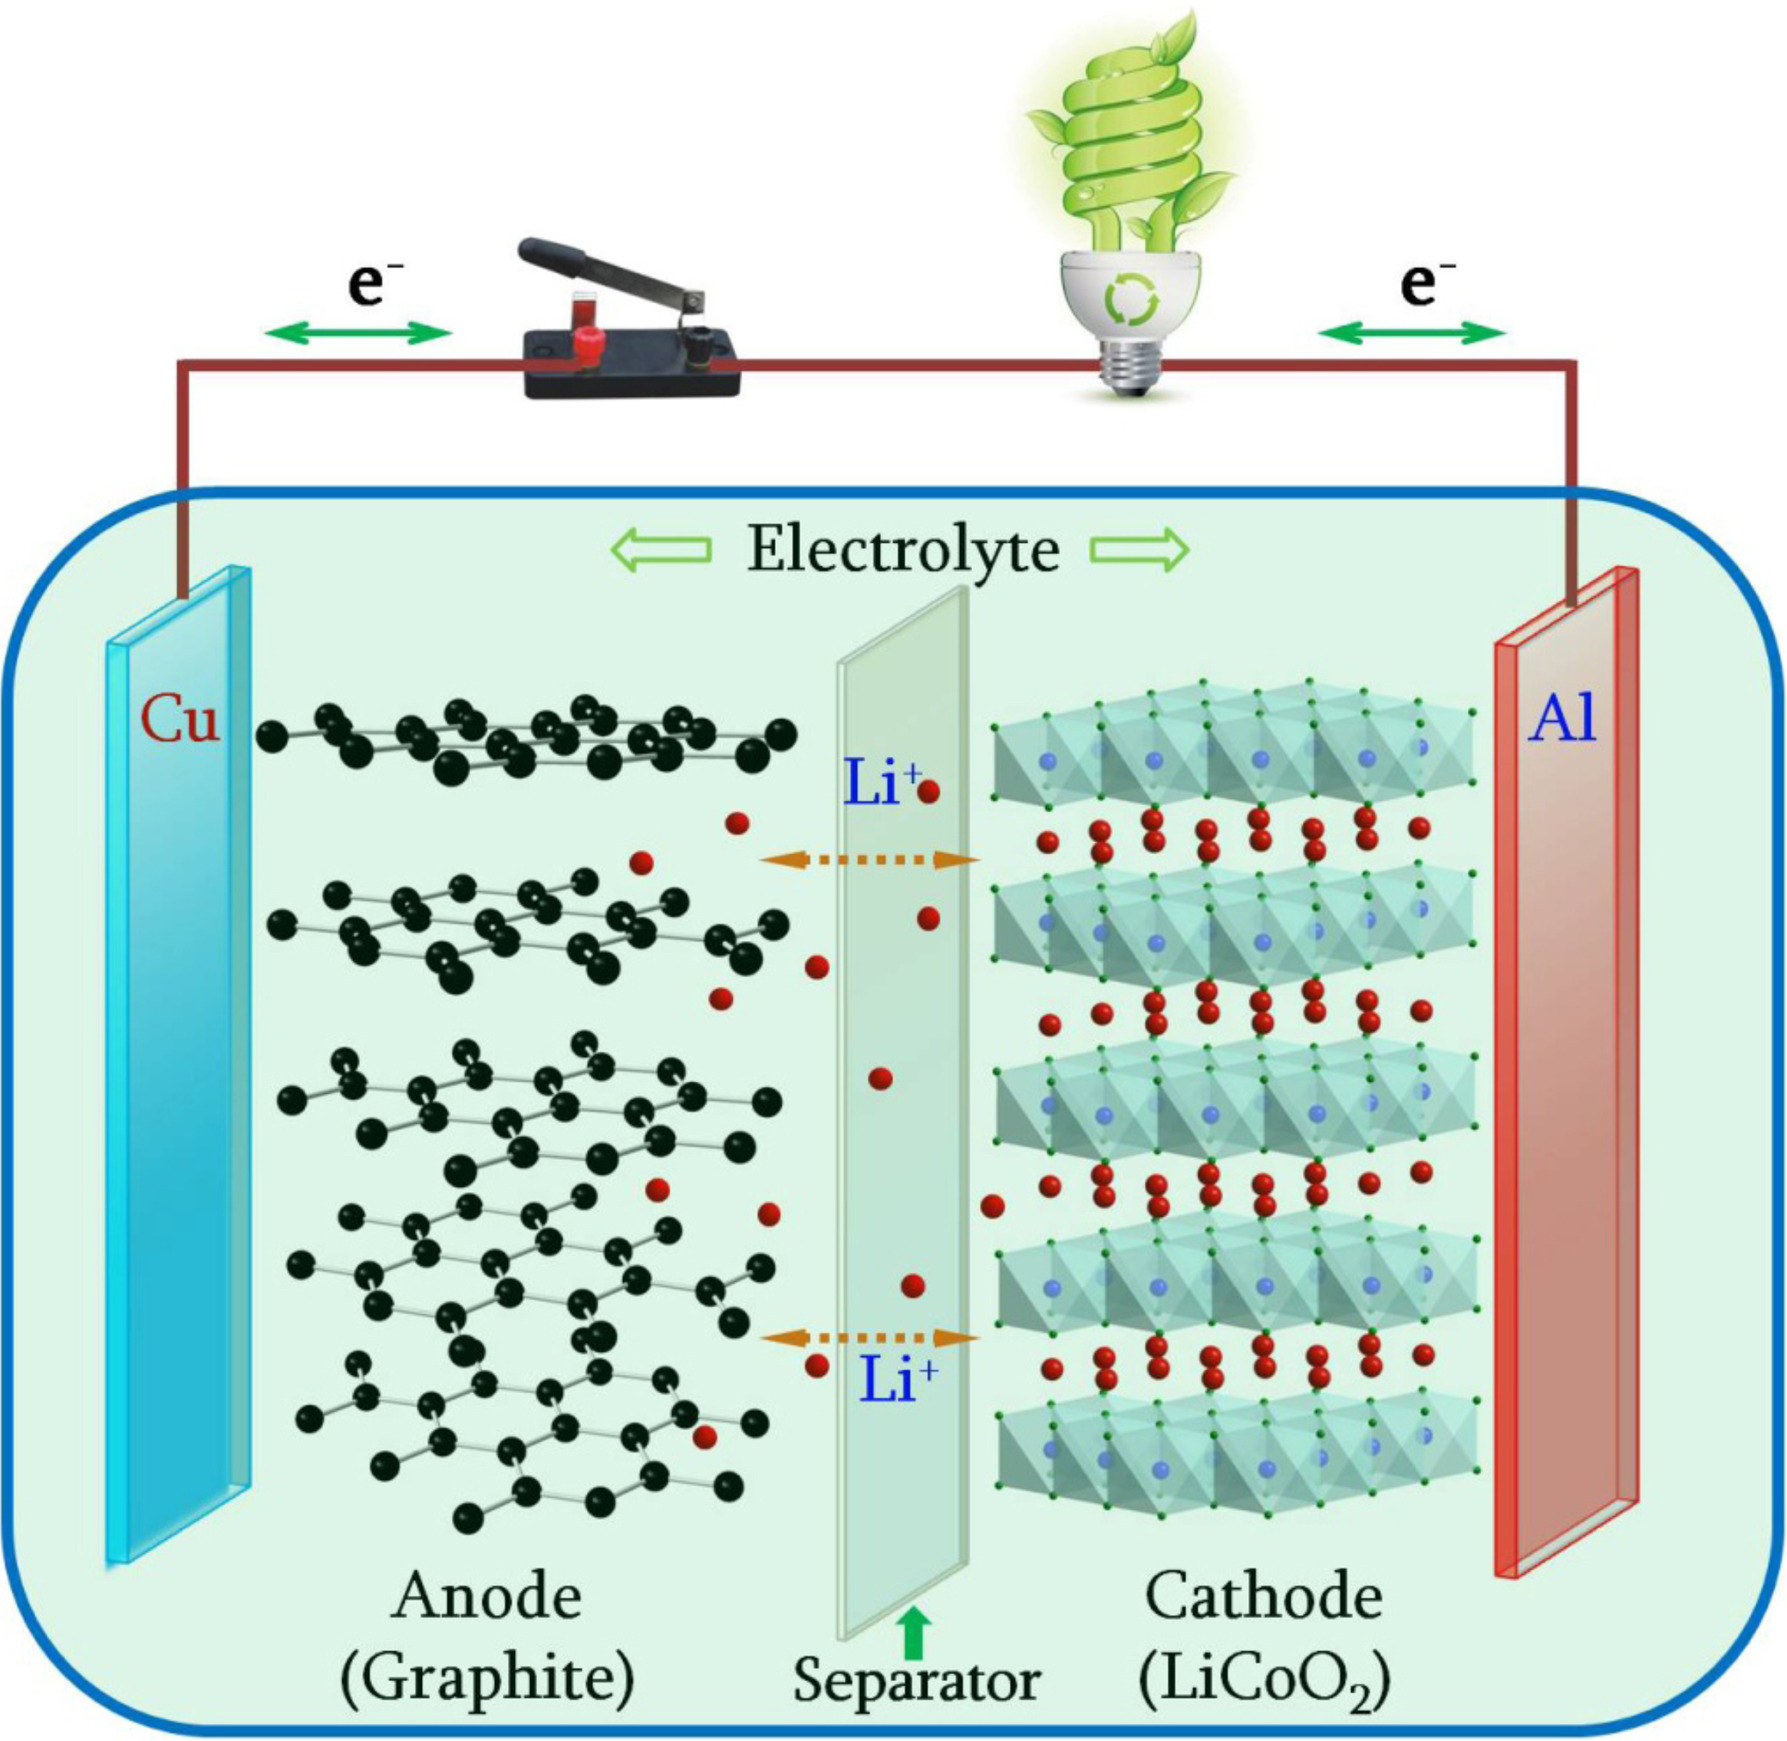
\includegraphics[scale=1]{LiIon3.png}
\caption{Bateria d'ió Liti \citep{liu_understanding_2016}.}
\label{fig:LiIon3}
\end{figure}

Podem definir el potencial estàndar d'una cel·la, $\Delta \varepsilon^{\circ}$, com al potencial pres en unes condicions determinades, que es fixen com a 1M per a tots els materials solubles, 1 atm per als gasos i, en el cas dels sòlids, la seva forma més estable a 25$^{\degree}$.
A partir del potencial podem calcular el treball elèctric fent
\[\Delta \varepsilon^{\circ} \times q = w_{elect}\]
Si la reacció és espontànea, el potencial $\Delta \varepsilon^{\circ}$ serà positiu.
Per tal de poder tabular els potencials de moltes substàncies, es va prendre la convenció d'assignar el potencial de 0 volt a la mitja reacció:
\[\ch{H2 (1 atm) <=> 2 H+ (1 M) + 2 e-}\]

\begin{exr}
La reacció que té lloc en una bateria d'ió liti com la de la imatge
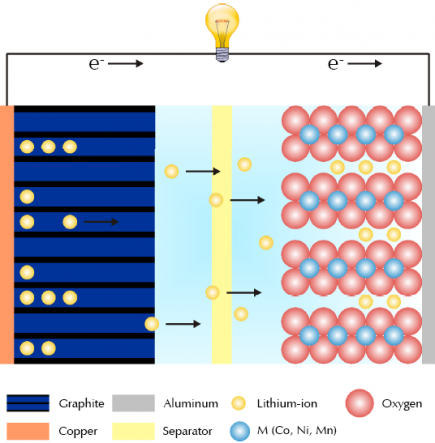
\includegraphics[scale=0.5]{LiIon.png}
és \ch{LiC6 + CoO2 <=> LiCoO2 + C6}. Escriu les dues mitges reaccions i fes-hi el balanç. Calcula el potencial de cel·la a partir de la $\Delta \varepsilon^{\circ}$ del \ch{Li+} (-3.0V) i del \ch{CoO2} (+1.1V).
Quins valors obtindries per a la reacció que tindria lloc en una bateria de Li i \ch{O2} ($\Delta \varepsilon^{\circ}$ de la reacció \ch{O2_{(g)} + 2 H+ + 2 e- -> H2O2_{(aq)}} és 0.3V).
\end{exr}

\subsection{Equació de Nernst}

El voltatge real d'una cel·la depèn de la concentració.
A partir de la $\Delta \varepsilon^{\circ}$ podem verue com, per a una reacció del tipus 
\[\ch{a A + b B <=> c C + d D}\]
el voltatge de la cel·la es calcularà fent
\[\Delta \varepsilon=\Delta \varepsilon^{\circ}-\frac{0.059}{n} \log \frac{[C]^c[D]^d}{[A]^a[B]^b}\] 
És fàcil veure que, en l'equilibri, $\Delta \varepsilon=0$.

\begin{exr}
Troba constant d'equilibri de la reacció \ch{2 Fe^{2+} + 3 I-  <=> 2 Fe ^{(2+)} + I3-}.
\end{exr}

\begin{exr}
Quina és la concentració en equilibri de \ch{Fe^{2+}} si posem una barra de ferro en una dissolució 1 M d'ions \ch{Zn^{2+}}?
\end{exr}

%\subsection{Valoracions REDOX}
%\subsection{Electròlisi}
%\subsection{Aplicacions electroquímiques}
